\documentclass[tikz]{standalone}
\usepackage{amsmath}
\begin{document}
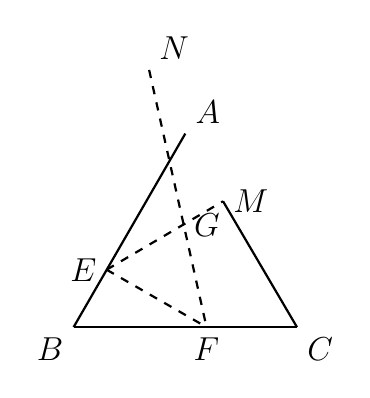
\begin{tikzpicture}[thick, font=\large, scale=0.01, yscale=-1]
  % 顶点与点坐标（已按原图比例换算，y 轴翻转）
  \coordinate (A) at (222,138);
  \coordinate (B) at (80,384);
  \coordinate (C) at (364,384);
  \coordinate (E) at (122,311);
  \coordinate (F) at (249,384);
  \coordinate (M) at (270,224);
  \coordinate (G) at (220,255);
  \coordinate (N) at (176,57);

  % 三角形实线：AB、BC（AC 中仅保留 MC 段，删除 AM 段）
  \draw (B) -- (A);
  \draw (B) -- (C);
  \draw (M) -- (C);

  % 虚线
  \draw[dashed] (N) -- (F);
  \draw[dashed] (E) -- (M);
  \draw[dashed] (E) -- (F);

  % 标签
  \node[above right] at (N) {$N$};
  \node[above right] at (A) {$A$};
  \node[right] at (M) {$M$};
  \node[right] at (G) {$G$};
  \node[left] at (E) {$E$};
  \node[below] at (F) {$F$};
  \node[below left] at (B) {$B$};
  \node[below right] at (C) {$C$};
\end{tikzpicture}
\end{document}
